\chapter{Reasoning Topologies, Hypothesis and Tests}
\label{ch:framework}

This chapter defines the three reasoning topologies as they are implemented, states what the hypothesis predicts, and describes the statistical tests used to confirm or reject it. The notation is deliberately small: $x$ is the serialized evidence, $y$ is a method's answer (the reported attack events with stages, plus a narrative), and each model call is written as $\mathrm{LLM}(\cdot)$.

\section{The Three Topologies}
\subsection{Chain-of-Thought}
CoT makes one model call over the whole evidence:
\begin{equation}
y=\mathrm{LLM}(x).
\end{equation}
The model reasons step by step inside that single generation. It cannot revisit an earlier step, and every part of $x$ competes for attention in one long context.

\subsection{Tree-of-Thoughts}
ToT samples $k=3$ candidate answers from the same prompt, asks the model to score each candidate against the evidence on a scale from 0 to 1, and keeps the best:
\begin{equation}
y_i=\mathrm{LLM}(x),\quad s_i=\mathrm{Score}(x,y_i)\in[0,1],\quad y=y_{i^\ast},\ \ i^\ast=\arg\max_i s_i .
\end{equation}
One generation call yields the three candidates and three scoring calls rate them, so a ToT run makes four calls. Candidates do not see each other, and everything found by a discarded candidate is lost.

\subsection{Graph-of-Thoughts}
GoT~\cite{besta2024got} models reasoning as a graph in which a node may have several parents. Our graph has four steps:
\begin{align}
&\text{Split:}      && x \rightarrow x_1,\dots,x_4 \quad(\text{four segments of similar text size}),\\
&\text{Generate:}   && z_i=\mathrm{LLM}(x_i),\quad i=1,\dots,4,\\
&\text{Aggregate:}  && a=\mathrm{LLM}(z_1,z_2,z_3,z_4)\quad(\text{many parents, one child}),\\
&\text{Refine:}     && y=\mathrm{LLM}(x,a).
\end{align}
Each segment is analysed without seeing the others, so the Aggregate call is the only place where findings from different parts of the log meet. Refine sees the full evidence together with the merged answer. In the v5 variant the Aggregate call also receives a short list of structural links between segments: an external address contacted from more than one segment, and a file written in one segment whose name appears in a process launched in another. A GoT run makes six calls (four, one, one), fewer when a log yields fewer segments. If the Refine output cannot be parsed, the merged answer is kept.

Figure~\ref{fig:topologies} contrasts the three structures and Table~\ref{tab:cost} gives their measured cost.

\begin{figure}[H]
\centering
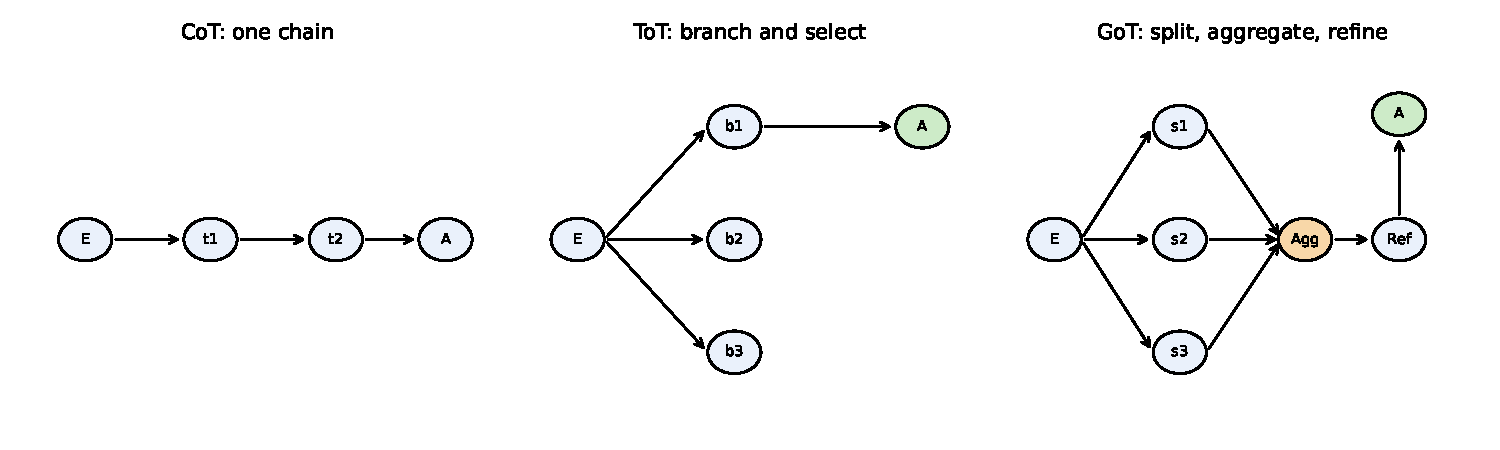
\includegraphics[width=0.95\textwidth]{fig_topologies}
\caption{The three reasoning topologies. E is the evidence, A the answer, Agg the Aggregate step and Ref the Refine step.}
\label{fig:topologies}
\end{figure}

\begin{table}[H]
\centering
\caption{Average cost per run in the baseline grid (21 runs per method).}
\label{tab:cost}
\small
\begin{tabular}{@{}lrrr@{}}
\toprule
\textbf{Method} & \textbf{LLM calls} & \textbf{Tokens} & \textbf{Wall clock (s)} \\
\midrule
CoT & 1.0 & 37{,}467 & 25.8 \\
ToT & 4.0 & 149{,}666 & 40.4 \\
GoT & 5.4 & 81{,}461 & 103.4 \\
\bottomrule
\end{tabular}
\end{table}

GoT uses fewer tokens than ToT because most of its calls read only a quarter of the evidence, but it takes the longest wall-clock time because its steps run one after another.

\section{Why Aggregation Should Help: the Formal Argument}
Besta et al.~\cite{besta2024got} define the \emph{volume} of a thought as the number of earlier thoughts from which it is reachable, that is, how much prior reasoning could have informed it. For $N$ thoughts and branching factor $k$:

\begin{table}[H]
\centering
\caption{Latency and volume of the final thought for each topology~\cite{besta2024got}.}
\label{tab:volume}
\small
\begin{tabular}{@{}lcc@{}}
\toprule
\textbf{Topology} & \textbf{Latency (longest path)} & \textbf{Volume of final thought} \\
\midrule
CoT & $N$ & $N$ \\
ToT & $\log_k N$ & $O(\log_k N)$ \\
GoT & $\log_k N$ & $N$ \\
\bottomrule
\end{tabular}
\end{table}

GoT is the only scheme with both low latency, like a tree, and full volume, like a chain, because its aggregation node is reachable from every independently reasoned segment, whereas a tree keeps only the one surviving path. This is why H1 predicts an advantage specific to aggregation and not merely from branching.

\section{What the Hypothesis Predicts}
\begin{enumerate}
\item \textbf{Main effect.} Stage recall of GoT exceeds that of ToT, which exceeds that of CoT, aggregated over scenarios and seeds, with the GoT--ToT gap statistically distinguishable. This isolates aggregation, because ToT already has branching and evaluation.
\item \textbf{Ablation control.} GoT with Aggregate outperforms GoT without Aggregate (independent segment answers, best one kept) at equal or larger call budget. This would separate aggregation from simply making more calls.
\item \textbf{Cost.} GoT is expected to cost the most. Cost is reported separately and is not part of the accuracy claim.
\end{enumerate}
H1 is rejected if GoT's stage recall is statistically indistinguishable from, or below, that of ToT and CoT.

\section{Tests Performed}
\label{sec:tests}
\paragraph{Paired topology comparison (prediction 1).} For a given experiment, each method is run on the same scenarios, models and seeds, so a run of one method can be paired with a run of another. For each pair of methods we form the per-cell differences $d_j=m_j(\text{A})-m_j(\text{B})$ of a metric $m$ (stage recall is the primary metric, event recall secondary) and apply the two-sided Wilcoxon signed-rank test~\cite{wilcoxon1945} to $d_j$. The null hypothesis is that the median difference is zero. We report the mean difference $\Delta$, the $p$-value and the number of pairs $n$. A comparison is called significant only at $p<0.05$. The test is non-parametric because scores are bounded and many are zero, and paired because scenario difficulty varies far more than method differences. Each seed of a scenario counts as one pair, which treats repeated runs as independent and makes the test somewhat anti-conservative. Because we test three comparisons on two metrics in five experiments (30 tests), we also state which results survive Bonferroni and Holm correction.

\paragraph{Paired variant comparison.} The same test compares an earlier and a later variant of the pipeline (for example before and after adding stage definitions) over matched (scenario, model, method, seed) cells.

\paragraph{Diagnostic checks.} Because a non-significant result cannot distinguish ``no effect'' from ``no power'', we also read raw outputs against ground truth. This produced a stage confusion matrix, a stage-label distribution per model, a split of results by input length, and a parse-success analysis (Chapter~\ref{ch:discussion}).

\paragraph{Not performed.} The ablation control of prediction 2 (GoT without Aggregate) was not run. The nearest experiment is v5, which changes what Aggregate receives, not whether it exists. A related control, segmented CoT, is proposed as future work (Chapter~\ref{ch:conclusion}).
